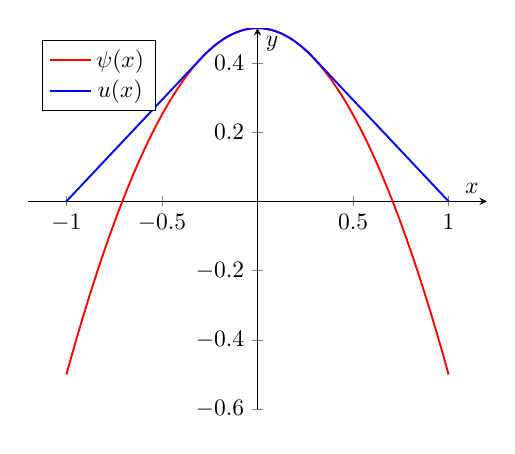
\begin{tikzpicture}[scale=0.85]
    \begin{axis}[
      axis lines = middle,
      xlabel = {$x$},
      ylabel = {$y$},
      domain = -1:1,
      samples = 100,
      xmin = -1.2,
      xmax = 1.2,
      ymin = -0.6,
      ymax = 0.5,
      legend pos = north west
    ]
      % Parameters
      \def\b{(2-sqrt(2))/2}
      \def\a{-\b}
      % Plot the obstacle function psi(x)
      \addplot[
        thick,
        red
      ] {0.5 - x^2};
      \addlegendentry{$\psi(x)$}
  
      % Plot u(x) in three pieces
      \addplot[
        thick,
        blue,
        domain=-1:\a
      ] {((.5 - \a*\a)/(\a + 1))*(x + 1)};

  
      \addplot[
        thick,
        blue,
        domain=\a:\b
      ] {0.5 - x^2};

  
      \addplot[
        thick,
        blue,
        domain=\b:1
      ] {-((.5 - \b*\b)/(1 - \b))*(x - 1)};
      \addlegendentry{$u(x)$}


    \end{axis}
  \end{tikzpicture}
  